\documentclass{beamer}

\usetheme{Singapore}
\usecolortheme{rose}

\usepackage[utf8]{inputenc}
\usepackage[vietnamese]{babel}

\setbeamertemplate{footline}[frame number]

% Adding todo notes
\usepackage{todonotes}
\presetkeys{todonotes}{inline}{}

% Add color text
\usepackage{xcolor}
\definecolor{olive}{rgb}{0.3, 0.4, .1}
\definecolor{fore}{RGB}{249,242,215}
\definecolor{back}{RGB}{51,51,51}
\definecolor{title}{RGB}{255,0,90}
\definecolor{dgreen}{rgb}{0.,0.6,0.}
\definecolor{gold}{rgb}{1.,0.84,0.}
\definecolor{JungleGreen}{cmyk}{0.99,0,0.52,0}
\definecolor{BlueGreen}{cmyk}{0.85,0,0.33,0}
\definecolor{RawSienna}{cmyk}{0,0.72,1,0.45}
\definecolor{Magenta}{cmyk}{0,1,0,0}

% Cấu hình table và nhập code
\usepackage{tabu,color,listings}
\definecolor{dkgreen}{rgb}{0,0.6,0}
\definecolor{gray}{rgb}{0.5,0.5,0.5}
\definecolor{mauve}{rgb}{0.58,0,0.82}
\lstset{inputpath=Filecodes}
\lstset{frame=none,
	language=[Sharp]C,
	aboveskip=3mm,
	belowskip=3mm,
	showstringspaces=false,
	columns=flexible,
	basicstyle={\small\ttfamily},
	numbers=none,
	numberstyle=\tiny\color{gray},
	keywordstyle=\color{blue},
	commentstyle=\color{dkgreen},
	stringstyle=\color{mauve},
	breaklines=true,
	breakatwhitespace=true,
	tabsize=3
}

% Sử dụng gói algorithm2e để viết thuật toán
\usepackage{algorithm2e}

% Tham chiếu tài liệu tham khảo
\usepackage[round]{natbib} 
\bibliographystyle{plainnat}

\title{ĐỘ TƯƠNG TỰ HÀNH VI CỦA CHƯƠNG TRÌNH VÀ THỰC NGHIỆM}
\author{Đỗ Đăng Khoa}
\institute{KHMT K19 -- ĐHQN}
\date{Quy Nhơn, 25--08--2017}

\begin{document}

\begin{frame}
  \titlepage
\end{frame}

\part{}

\begin{frame}
  \frametitle{Nội dung}
  \tableofcontents{}
\end{frame}

\section{Giới thiệu}
\begin{frame}
  \frametitle{Học trực tuyến}
  \begin{minipage}{0.39\linewidth}
    
\includegraphics[width=0.9\linewidth]{images/topMOOC.png} 
  \end{minipage} \pause	
  \hfill
  \begin{minipage}{0.59\linewidth}
    \begin{itemize}
    \item Một số vấn đề
      \begin{itemize}
      \item Người dạy ít, người học đông
      \item Tốn thời gian tìm hiểu mã lệnh 
      \item Đánh giá, xếp hạng
      \end{itemize} \pause
    \item Giải pháp
      \begin{itemize}
      \item Công cụ hỗ trợ tự động 
      	\begin{itemize}
      	\item So sánh hai giải pháp
      	\item Tương đương hay tương tự      	
    	\end{itemize}
      \end{itemize}
    \end{itemize} \pause
	\begin{block}{Vấn đề cốt lõi}
		Đo được độ tương tự về hành vi giữa hai chương trình
	\end{block}
  \end{minipage}
\end{frame}

\begin{frame}
  \frametitle{Một số nghiên cứu liên quan}  
	%\todo{Phải nói rõ người ta làm thế nào, mình khác người thế nào? ghép trích dẫn cho gọn}
  \begin{itemize}
  \item Xếp hạng tự động
    \begin{itemize}
    \item \cite{alur2013automated} sử dụng khái niệm về độ tương tự về ngữ nghĩa dùng cho automat hữu hạn đơn định; giải pháp luận văn dùng cho các chương trình máy tính    
    \end{itemize}
  \item Kiểm tra sự tương đương giữa hai chương trình
    \begin{itemize}
    \item \cite{bates1993incremental} sử dụng đồ thị phụ thuộc; giải pháp luận văn còn có thể đo được độ tương tự. 
    \item \cite{jiang2009automatic} sử dụng các phép thử ngẫu nhiên tương tự phép đo RS trong luận văn, khác phép đo SSE và PSE
    \end{itemize}
  \item Phát hiện đạo code
    \begin{itemize}
    \item \cite{komondoor2001using} sử dụng đồ thị phụ thuộc của chương trình, tính toán độ tương tự bằng cách phân tích tĩnh các đoạn mã lệnh; tiếp cận trong luận văn thực thi chương trình để sinh ra các cặp dữ liệu vào/ra.
    \end{itemize}
  \end{itemize}

\end{frame}

\begin{frame}
  \frametitle{Dynamic Symbolic Execution}
%  \todo{Đọc lại thật kỹ DSE, diễn đạt lại cho tốt hơn, giải thích ví dụ chưa ổn, hãy cẩn trọng}
  \begin{itemize}
  \item Ý tưởng chính
    \begin{itemize}
    \item Dựa trên kiểu dữ liệu đầu vào của chương trình
    \item DSE tạo ra các giá trị đầu vào cụ thể và thực thi chương trình 
    \item Ghi nhận ràng buộc tại các nút rẽ nhánh
    \item Phủ định lại ràng buộc, sinh ra giá trị đầu vào mới
    \item Quá trình thực thi lặp lại
    \end{itemize}
  \end{itemize} \pause
	
  \begin{block}{Cách thức hoạt động}
    \begin{minipage}[T]{0.40\linewidth}
      \lstinputlisting[basicstyle=\footnotesize]{test_me.cs}
    \end{minipage}
    \hfill    
    \begin{minipage}[T]{0.55\linewidth}
		{\footnotesize\centering
		\begin{tabular}{  m{4em} | m{4em} | m{4em}  }
		concrete state & symbolic state & path condition \\ 
		\hline
		$ x = 0 $ & $ x = x_{0} $ & $ x_{0} != 10 $ \\  
		\hline
		$ x = 10 $ & $ x = x_{0} $ & $ x_{0} == 10 $ \\ 		
		\end{tabular}
		\\ \pause
		Kết quả sau hai lần thực thi: $ 0, 10 $ 
		}
    \end{minipage}
  \end{block}
	
\end{frame}

\section{Sự tương tự về hành vi chương trình}

\begin{frame}
  \frametitle{Hai chương trình tương đương}
%  \todo{Viền code cho đẹp hơn}
  \begin{minipage}[t]{0.45\linewidth}
    \lstinputlisting[basicstyle=\footnotesize]{SwitchCase.cs}
  \end{minipage}
  \hfill\vrule\hfill
  \begin{minipage}[t]{0.45\linewidth}
    \lstinputlisting[basicstyle=\footnotesize]{IfElse.cs}
  \end{minipage}
  \begin{itemize}
  \item Cùng tham số đầu vào $ x $ kiểu \texttt{int}
  \item Trả về giá trị $ y $ phụ thuộc vào $ x $
  \item Cấu trúc khác nhau
  \end{itemize}
\end{frame}


\begin{frame}
  \frametitle{Thực thi của một chương trình}
%  \todo{Tìm cách trình bày lại tất cả các định nghĩa cho đẹp hơn, dễ đọc hơn}
  \begin{itemize}
  	\item Cho $P$ là một chương trình, $I$ là tập hợp các trị đầu vào của $P$, 
  	$O$ là tập hợp các giá trị đầu ra của $P$. 
  	Thực thi chương trình P là ánh xạ: 
  	\[exec: P \times I \rightarrow O\]
  	\item Với $i \in I$, $o \in O$ thực thi chương trình $P$ trên
  	$i$ ta thu được giá trị đầu ra tương ứng $o = exec(P, i)$.
  \end{itemize}  
\end{frame}


\begin{frame}
  \frametitle{Tương đương về hành vi của 2 chương trình}
  \begin{itemize}
  	\item Cho $P_{1}$ và $P_{2}$ là hai chương trình có cùng miền các giá trị
  	đầu vào $I$. 
  	\item Hai chương trình này được gọi là tương đương khi và chỉ
  	khi thực thi của chúng giống nhau trên mọi giá trị đầu vào trên $I$,
  	Ký hiệu: \[exec(P_{1}, I) = exec(P_{2}, I).\]
  \end{itemize}
 
\end{frame}


\begin{frame}
  \frametitle{Sự khác biệt hành vi}
  \begin{itemize}
  	\item Cho $P_{1}$ và $P_{2}$ là hai chương trình có cùng miền các giá trị
  	đầu vào $I$. 
  	\item Hai chương trình này được xem là có sự khác biệt về
  	hành vi khi và chỉ khi thực thi của chúng khác nhau trên một vài giá
  	trị đầu vào $i \in I$, ký hiệu là: \[exec(P_{1}, I) \neq exec(P_{2}, I)\]
  \end{itemize}

\end{frame}


\begin{frame}
  \frametitle{Độ tương tự về hành vi}
  \begin{itemize}
  	\item  Cho $P_{1}$ và $P_{2}$ là hai chương trình có cùng miền giá trị đầu
  	vào $I$. 
  	\item Gọi $I_{s} \subseteq I$ là tập con của $I$ sao cho
  	$exec(P_{1}, I_{s}) = exec(P_{2}, I_{s})$ và
  	$\forall j \in I \setminus I_{s}, exec(P_{1}, j) \neq exec(P_{2},
  	j)$. Khi đó, độ tương tự về hành vi giữa $P_1$ và $P_2$ là $|I_s|/|I|$.
  \end{itemize}
\end{frame}


\section{Một số phép đo độ tương tự}
\begin{frame}
  \frametitle{Lấy mẫu ngẫu nhiên}
  \begin{itemize}  	
  	\item Lấy ngẫu nhiên một số giá trị trên miền vào \\(\emph{Random
  		Sampling -- RS})
  	\item Tính số lượng giá trị hai chương trình
  	thực thi giống nhau
  	\item Mô tả hình thức:
  	\begin{itemize}
  		\item $P_{1}$ và $P_{2}$ là hai chương trình có cùng miền giá trị đầu
  		vào $I$
  		\item $I_{s}$ là tập con ngẫu nhiên của $I$
  		\item $I_{a}$ là tập con
  		$I_{s}$ sao cho $exec(P_{1}, I_a) = exec(P_{2}, I_a)$
  		\item Và $\forall j \in I_{s} \setminus I_{a}$, thì
  		$exec(P_{1}, j) \neq exec(P_{2}, j)$
  		\item $M_{RS}(P_{1}, P_{2}) = \left|I_{a}\right| \diagup
  		\left|I_{s}\right| $.
  	\end{itemize}
  \end{itemize}
\end{frame}


\begin{frame}
  \frametitle{Thuật toán phép đo RS}
%  \todo{Tìm cách tách phần input và các bước thực hiện để rõ hơn, trong tất cả các thuật toán}
  \begin{algorithm}[H]
  	\KwIn{
  		$P_{1}, P_{2}$ hai chương trình cần đo độ tương tự có cùng miền giá trị vào $I$\;	  	
  	}  	
	Set $I_{s} = Random(I)$ \;
	Set $I_{a} = \emptyset$\;
  	\For{$i \in I_s$}
  	{  			
		\eIf{$ (exec(P_{1}, i) = exec(P_{2}, i)) $}{
			$I_{a} = I_{a} \cup i$\;
		}{
			Next\;
		}
  	}
	\KwOut{$M_{RS}(P_{1}, P_{2}) = \left|I_{a}\right| \diagup
		\left|I_{s}\right| $.}
  \end{algorithm}
\end{frame}


\begin{frame}
  \frametitle{DSE trên chương trình tham chiếu}
%  \todo{Việc tìm tập dữ liệu thử do DSE làm}
  \begin{itemize}
  	\item Việc tìm tập dữ liệu thử do DSE làm
  	\item Áp dụng DSE trên chương trình tham chiếu
  	\\ (\emph{Single program Symbolic Execution -- SSE})
  	\item Phân tích các câu lệnh chương trình tham chiếu
  	\item Xác định tập dữ liệu thử
  	\item Mô tả hình thức
  	\begin{itemize}
	\item $P_{1}$ và $P_{2}$ là hai chương trình có cùng miền giá trị đầu
	vào $I$
	\item $P_{1}$ là chương trình tham chiếu
	\item $I_{s} = DSE(P_{1})$
	\item $I_{a} \subseteq I_s$ sao cho
	$exec(P_{1}, I_a) = exec(P_{2}, I_a)$
	\item $\forall j \in I_{s} \setminus I_{a}, exec(P_{1}, j) \neq
	exec(P_{2}, j)$
	\item $M_{SSE}(P_{1}, P_{2}) = \left|I_{a}\right| \diagup
	\left|I_{s}\right| $.
  	\end{itemize}
  \end{itemize}
\end{frame}


\begin{frame}
  \frametitle{Thuật toán phép đo SSE}
  \begin{algorithm}[H]
  	\KwIn{
  		$P_{1}, P_{2}:$ hai chương trình cần đo tương tự có cùng miền giá trị vào $I$; $P_1$ là chương trình tham chiếu\; 
  	}  	
  	Set $I_{s} = DSE(P_{1})$ \;
  	Set $I_{a} = \emptyset$ \;
  	\For{$i \in I_{s}$}
  	{  			
  		\eIf{$ (exec(P_{1}, i) = exec(P_{2}, i)) $}{
  			$I_{a} = I_{a} \cup i$\;
  		}{
  			Next\;
  		}
  	}
  	\KwOut{$M_{SSE}(P_{1}, P_{2}) = \left|I_{a}\right| \diagup
  		\left|I_{s}\right| $.}
  \end{algorithm}
\end{frame}


\begin{frame}
  \frametitle{DSE trên chương trình hợp thành}
%  \todo{Tách riêng ý về chương trình hợp thành, sau đó nói về DSE trên nó}
  \begin{itemize}  	
  	\item Mô hình hóa chương trình hợp thành:
  	\begin{itemize}
  		\item $P_1$ và $P_2$ là hai chương trình có cùng miền vào $I$
  		\item $P_1$ là chương trình tham chiếu
  		\item $P_c = P_1 \oplus P_2$ có dạng
  		$assert(exec(P_{1}, I) = exec(P_{2}, I))$
  		\item  $assert(\dots)$ là hàm đánh giá biểu thức đúng hay sai
  		\item Ký hiệu $exec(P_c,i) = \top$ để chỉ
  		chương trình hợp thành $P_c$ thỏa hàm đánh giá, cũng có nghĩa là hai
  		chương trình thành phần thực thi giống nhau trên đầu vào $i$.  				
  	\end{itemize}
  \item Áp dụng DSE trên chương trình hợp thành xác định tập dữ liệu thử 
  \end{itemize}
\end{frame}


\begin{frame}
  \frametitle{Thuật toán phép đo PSE}
  \begin{algorithm}[H]
  	\KwIn{
  		$P_{1}, P_{2}$ là hai chương trình cần đo tương tự, có cùng miền giá trị đầu
  		vào $I$; $P_1$ là chương trình tham chiếu\;  	
  	}  	
  	$P_{3} = P_1 \oplus P_2$\;
  	Set $I_{s} = DSE(P_{3})$ \;
  	Set $I_{a} = \emptyset$ \;
  	\For{$i \in I_{s}$}
  	{  			
  		\eIf{$ (exec(P_{1}, i) = exec(P_{2}, i)) $}{
  			$I_{a} = I_{a} \cup i$\;
  		}{
  			Next\;
  		}
  	}
  	\KwOut{$M_{PSE}(P_{1}, P_{2}) = \left|I_{a}\right| \diagup
  		\left|I_{s}\right| $.}
  \end{algorithm}
\end{frame}


\section{Thực nghiệm}

\begin{frame}
  \frametitle{Nguồn dữ liệu và các công cụ sử dụng}
%  \todo{Ghép slide Nguồn dữ liệu và Công cụ thành 2 blocks}
  \begin{block}{Nguồn dữ liệu}
  	\begin{itemize}
  		\item Trò chơi Code Hunt
  		\begin{itemize}
  			\item 24 câu hỏi
  			\item 250 người sử dụng
  			\item Chương trình do sinh viên viết
  		\end{itemize}
  		\item Tự xây dựng
  	\end{itemize}
  \end{block} \pause
  \begin{block}{Các công cụ sử dụng}
  	\begin{itemize}
  		\item Microsoft Visual Studio
  		\item Công cụ sinh dữ liệu thử PEX
  		\begin{itemize}
  			\item Sản phẩm của Microsoft
  			\item Dựa trên kỹ thuật DSE
  			\item Tích hợp như một Add-in
  		\end{itemize}
  	\end{itemize}
  \end{block}
\end{frame}

\begin{frame}
  \frametitle{Kết quả thực nghiệm}
%  \todo{Sửa lại title cụ thể hơn cho mỗi slide}
  \centering
  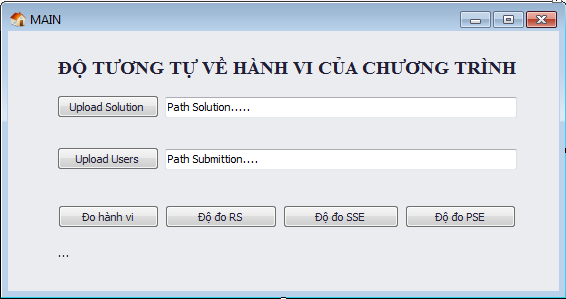
\includegraphics[width=0.8\linewidth]{images/main.png}
  
\end{frame}

\begin{frame}
\frametitle{Kết quả phép đo RS}
\centering
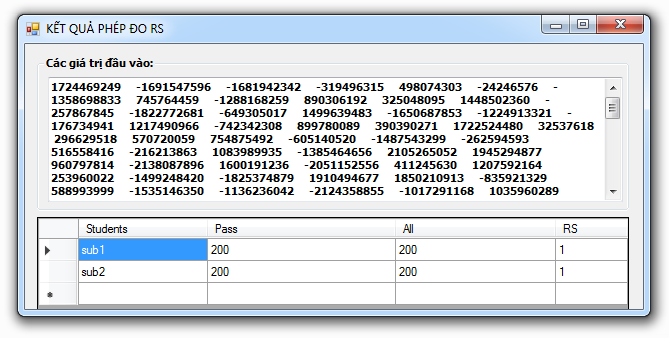
\includegraphics[width=0.8\linewidth]{images/kq_rs.png}
\end{frame}

\begin{frame}
\frametitle{Kết quả phép đo SSE}
%  \todo{Nên tách từng thực nghiệm, mỗi cái cần giải thích dữ liệu liên quan}
\centering
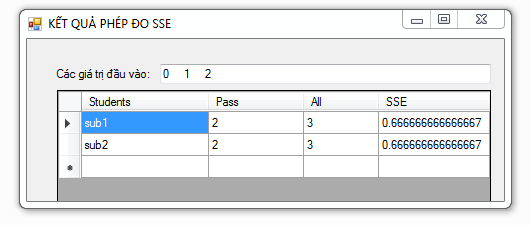
\includegraphics[width=0.8\linewidth]{images/kq_sse.png} 
\end{frame}

\begin{frame}
\frametitle{Kết quả phép đo PSE}
\centering
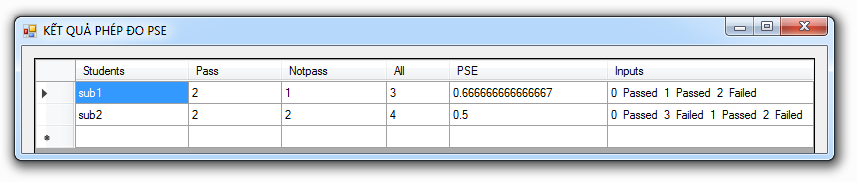
\includegraphics[width=0.8\linewidth]{images/kq_pse.png}
\end{frame}

\begin{frame}
  \frametitle{Kết luận}
%  \todo{Còn thiếu, đầu tiên phải nói những thứ mình làm}
	
  \begin{itemize}
  	\item Kết quả đạt được
  	\begin{itemize}
  		\item Kiến thức cơ sở
  		\item Kỹ thuật Dynamic symbolic execution
  		\item Kỹ thuật các phép đo RS, SSE, PSE
  		\item Ứng dụng lý thuyết, xây dựng ứng dụng
  	\end{itemize} \pause
  	\item Hướng phát triển
  	\begin{itemize}
  		\item Cải tiến các phép đo để kết quả được chính xác hơn
  		\item Tích hợp thêm một số ngôn ngữ Java, C++...
  	\end{itemize} \pause
  	\item Khả năng áp dụng
  	\begin{itemize}
  		\item Đánh giá tiến bộ trong lập trình
  		\item Xếp hạng tự động
  		\item Gợi ý giải pháp lập trình
  	\end{itemize}
  \end{itemize}
\end{frame}


\begin{frame}
  \frametitle{Tài liệu tham khảo}
%  \todo{Điều chỉnh style cho gọn hơn, đẹp hơn, font chữ nhỏ hơn cho vừa slide}
  \bibliographystyle{plain}
  {\footnotesize\bibliography{biblio}}
\end{frame}


\part{}

\begin{frame}
%  \todo{Sửa lại cho lịch sự hơn}
%  \todo{Sau khi hoàn thành hãy thêm hiệu ứng cho một số slides}
  \begin{center}
    \begin{Huge}
      \textcolor{BlueGreen}{\textbf{XIN CẢM ƠN}}
    \end{Huge}
\end{center}

\end{frame}

% Tài liệu tham khảo

\end{document}



%%% Local Variables:
%%% mode: latex
%%% TeX-master: t
%%% End:
